\chapter{Polynomials: The Structure Behind Equations}

\section{Three Measurements at a Skatepark}

A new skatepark on the south side of town has a launch ramp that sends skateboarders airborne. Its designer, Zhou, has drawn the flight path: a rider leaves the ramp's edge, traces an arc through the air, and lands on a descending slope. This arc cannot be drawn casually. The landing must fall on the gentlest part of the slope, or the rider could suffer anything from a tumble to a serious accident.

Put the site into a coordinate system, using the skill from Chapter 4: take the launch point as the origin, the horizontal direction as the $x$-axis, and the vertical direction as the $y$-axis, with metres as units. Zhou knows that, ignoring air resistance, the flight path is always a quadratic curve, described by
\[
y = ax^2 + bx + c
\]
for three numbers $a$, $b$, and $c$ yet to be determined. Such expressions appear everywhere: the arc of a fountain's stream, the path of a basketball shot, and the shape of a suspension bridge's main cable all belong to the same mathematical family. The difficulty is that the instruments have measured only three points on the path: the launch position $(0, 2)$, a point in the air $(1, 5)$, and the chosen safe landing point $(4, 2)$.

There are now two questions. First, does a quadratic curve pass through all three points, and if so, is it unique? Second, once the trajectory is determined, at what horizontal positions is the rider exactly $3$ metres high? That means solving $ax^2+bx+c=3$, or finding where the curve meets a horizontal line.

Make an intuitive guess first. Three conditions determine three unknowns, so perhaps a solution exists and is probably unique. That intuition is correct, but explaining why requires this chapter's tools. You may also think solving $ax^2+bx+c=3$ simply means applying the quadratic formula. But what if the discriminant is negative? Is the problem wrong, or is mathematics hinting at something?

These two questions launch our chapter. We will study an expression like $ax^2+bx+c$ as a building with internal structure, asking how its components (factors), foundations (roots), and number of storeys (degree) determine its behaviour. Then we will return to the skatepark to ask whether three points can recover a rule. Finally, we will confront the negative discriminant, which will lead us into a whole new world of numbers.

\section{Trying Intuition: Two Easy Traps}

When asked for a curve through three points, the natural approach is to guess. Try $y = -x^2 + 4x + 2$: at $x=0$, $y=2$, correct; at $x=1$, $y=5$, correct again; at $x=4$, $y = -16+16+2 = 2$, all correct! We got lucky this time. Change the points, though, and guessing becomes difficult. We cannot rely on luck every time. We need a method guaranteed to succeed that also proves uniqueness; later in the chapter we will find one.

Intuition about equations can stumble too. Many students memorize that the graph's intersections with the $x$-axis are the equation's roots, then infer two plausible-sounding claims:

\begin{itemize}
\item The equation has as many roots as the curve has encounters with the $x$-axis.
\item If the graph does not meet the $x$-axis, the equation is meaningless.
\end{itemize}

The first misses a subtle possibility: the curve can touch the $x$-axis and bounce back without crossing it, as $y=(x-1)^2$ does at $x=1$. The equation then has only one root, but that root occupies two places. The second is more dangerous: the graph associated with $x^2+1=0$ indeed cannot reach the $x$-axis, yet by this chapter's end we will see that the equation is meaningful and prompted one of the most important expansions of the number system in mathematical history.

\begin{fanli}
``A quadratic equation either has two roots or has no real roots.'' Wrong. $x^2-2x+1=0$ has only the root $x=1$, but it is repeated: the left side is $(x-1)^2$, where the factor $x-1$ appears twice. Saying only ``one root'' loses structural information; ``one double root'' is more precise. When reading a graph, remember that touching the $x$-axis tangentially and crossing the $x$-axis are fundamentally different encounters.
\end{fanli}

Both failures teach the same lesson: looking only at the answer is insufficient. We must take the expression apart and inspect its structure. Let us turn that dismantling into a formal tool.

\section{Expressions as Buildings: Polynomials, Degree, and Roots}

Take apart $3x^2-4x+1$, and you find several blocks added together: $3x^2$, $-4x$, and $1$. Each is a number multiplied by a power of $x$ (we can regard $1$ as $1\cdot x^0$). Such expressions are extremely convenient: they can be added and multiplied, and the results remain in the same family, like Lego bricks that stay within the system however you assemble them. To discuss these objects repeatedly, we give them a name.

\begin{dingyi}[Polynomial]
An expression of the form
\[
a_n x^n + a_{n-1} x^{n-1} + \cdots + a_1 x + a_0
\]
is called a \textbf{polynomial} in $x$, where $a_n, a_{n-1}, \ldots, a_0$ are fixed numbers called \textbf{coefficients}, and $n$ is a nonnegative integer. If $a_n \neq 0$, its \textbf{degree} is $n$, and $a_n$ is the \textbf{leading coefficient}.
\end{dingyi}

\begin{shuyu}{Degree}
Intuition: the exponent of the polynomial's fastest-growing term, determining the expression's character when $x$ is large.

Formal definition: the highest exponent of a term with nonzero coefficient.

Example: $x^3-7x+6$ has degree $3$; the constant $5$, or $5x^0$, has degree $0$.
\end{shuyu}

\begin{shuyu}{Root}
Intuition: an input that makes the polynomial zero; on the graph, a position where the curve meets the $x$-axis.

Formal definition: if a number $r$ satisfies $f(r)=0$, then $r$ is a root of the polynomial $f(x)$.

Example: $1$ and $3$ are roots of $x^2-4x+3$, because both give $0$ when substituted.
\end{shuyu}

Why invent a special word, degree? Because it acts like a building's storey count, largely determining its broad features. A degree-one polynomial has a straight-line graph, with one end rising and the other falling. A quadratic has a parabola; a cubic resembles a twisted ribbon, diving at one end and emerging at the other. Degree also answers a question that troubled ancient mathematicians: how many solutions can an equation have at most?

Polynomials also deserve study because they are simple enough and versatile enough. Simple, because evaluating them requires only multiplication and addition, with no elaborate operations---exactly the expressions computers like best. Versatile, because later, in Chapters 11 and 12, we will see that even apparently unrelated functions such as $\sin x$ and $\mathrm{e}^x$ can be approximated as closely as we like by infinitely long polynomials. Understanding polynomials lays foundations for the whole world of functions.

Roots weld algebra to geometry: solving $f(x)=0$ is equivalent to finding the intersections of $y=f(x)$ with the $x$-axis. The same object has an algebraic face and a geometrical face, and we can switch between them at will.

Now return to taking expressions apart. We can write $x^2-4x+3$ as $(x-1)(x-3)$. Once factored, its roots almost jump out: a product is zero if and only if at least one factor is zero, so the roots are $1$ and $3$. Conversely, knowing the roots $1$ and $3$ immediately suggests the factors $x-1$ and $x-3$. This translation between roots and factors deserves to become a theorem.

\section{The Factor Theorem: Translating Roots into Factors}

\begin{dingli}[The Factor Theorem]
Let $f(x)$ be a polynomial and $a$ a number. Then $a$ is a root of $f(x)$ if and only if $x-a$ is a factor of $f(x)$, meaning that some polynomial $q(x)$ satisfies
\[
f(x) = (x-a)\,q(x).
\]
\end{dingli}

\begin{proof}
Check the two directions separately.

(If $x-a$ is a factor.) Suppose $f(x)=(x-a)q(x)$. Substitute $x=a$: the first factor becomes $a-a=0$, and zero times any number is zero. Thus $f(a)=0$, so $a$ is a root.

(If $a$ is a root.) Recall division with remainder from primary school: $17$ divided by $5$ has quotient $3$ and remainder $2$, so $17 = 5\times 3 + 2$, with the remainder smaller than the divisor. Polynomials have an analogous division. Dividing $f(x)$ by the linear expression $x-a$ gives
\[
f(x) = (x-a)\,q(x) + r,
\]
where the remainder $r$ must have degree less than the degree $1$ of the divisor $x-a$, so $r$ can only be a constant. Substitute $x=a$. The left side is $f(a)=0$ because $a$ is a root; the first term on the right disappears, leaving $r$. Hence $r=0$, so $f(x) = (x-a)q(x)$ and $x-a$ is indeed a factor.
\end{proof}

\begin{li}
Verify that $x=2$ is a root of $f(x)=x^3-7x+6$ and factor the polynomial completely. Substitution gives $f(2)=8-14+6=0$, so it is a root and $x-2$ is a factor. Division, or patient trial, gives
\[
x^3-7x+6 = (x-2)(x^2+2x-3) = (x-2)(x-1)(x+3).
\]
The three roots are immediately visible: $2$, $1$, and $-3$. Once one root is found, solving a cubic has been reduced to solving a quadratic.
\end{li}

How exactly does the division work? Almost like long division with integers. Divide $x^3-7x+6$ by $x-2$. Start with the highest power, $x^3$: what power of $x$ multiplying $x-2$ supplies that term? The first quotient term is $x^2$. Multiply back to get $x^3-2x^2$ and subtract, leaving $2x^2-7x+6$. For $2x^2$, the next quotient term is $2x$; multiplying back gives $2x^2-4x$, and subtracting leaves $-3x+6$. The final quotient term is $-3$, whose product is $-3x+6$; subtraction clears everything, leaving remainder $0$. A zero remainder is another way to say that $2$ is a root. Divide using a number that is not a root and a small piece remains. That piece is exactly the function value, as the remainder theorem in Further Climbing explains.

This reduction in degree is powerful and repeatable, so an important result comes almost for free:

\begin{tuilun}
A polynomial of degree $n$ has at most $n$ distinct real roots.
\end{tuilun}

\begin{proof}
Every root $a$ supplies a linear factor $x-a$ by the factor theorem, splitting the polynomial as $(x-a)q(x)$ with $q(x)$ of degree $n-1$. Finding a root of $q(x)$ splits off another linear factor. Each step reduces the remaining degree by one. After at most $n$ steps it reaches $0$, leaving a constant with no further roots to split off. Thus there are at most $n$ distinct roots.
\end{proof}

\begin{zhu}
``At most'' is essential. $x^2+1$ has degree two but no real roots. Degree gives an \emph{upper bound}, not a guarantee. We will return to this gap at the chapter's end.
\end{zhu}

\section{Vieta's Relations: Hearing the Roots Without Factoring}

Factoring is satisfying, but sometimes the coefficients make it awkward, and sometimes complete factorization is unnecessary. Can we learn something about roots without solving the equation?

For quadratics we can, in a particularly elegant way. Let the roots of $x^2+bx+c=0$ be $\alpha$ and $\beta$, possibly equal. The factor theorem gives
\[
x^2+bx+c = (x-\alpha)(x-\beta).
\]
Expand the right side:
\[
(x-\alpha)(x-\beta) = x^2 - (\alpha+\beta)x + \alpha\beta.
\]
The two sides are the same polynomial, so corresponding coefficients must match. We obtain:

\begin{dingli}[Vieta's Relations for Quadratics]
If $\alpha$ and $\beta$ are the roots of $x^2+bx+c=0$, then
\[
\alpha+\beta = -b, \qquad \alpha\beta = c.
\]
For the general form $ax^2+bx+c=0$ with $a\neq 0$, divide both sides by $a$ to reach the preceding case, giving $\alpha+\beta=-\dfrac{b}{a}$ and $\alpha\beta=\dfrac{c}{a}$.
\end{dingli}

\begin{li}
Without solving $x^2-7x+12=0$, we know its roots sum to $7$ and multiply to $12$. Which two numbers have sum $7$ and product $12$? $3$ and $4$. Now consider $x^2+x+1=0$. If it has real roots, they sum to $-1$ and multiply to $1$. A positive product means the two real numbers have the same sign; a negative sum means both must be negative. But for two negative numbers whose product is $1$, the closest possibility is $-1$ and $-1$, whose sum is $-2$---a little short of the required $-1$. This shortfall is no coincidence; the chapter's ending will explain it.
\end{li}

The real value of Vieta's relations is obtaining information at a distance: the coefficients are \textbf{symmetric functions} of the roots. $\alpha+\beta$ and $\alpha\beta$ share a feature: swapping $\alpha$ and $\beta$ leaves their values unchanged. Coefficients see only symmetric information about the roots; they cannot report what they do not see, such as which root is larger. Remember the word symmetry: it is one of the keys to the next chapter. These relations are named after the sixteenth-century French mathematician Vieta. His contribution went beyond the two formulas: he began using letters systematically for known and unknown quantities. That notation made it possible to study all equations instead of solving them one at a time.

Cubic and quartic equations have Vieta relations too. For $x^3+px^2+qx+r=0$, the three roots sum to $-p$, their pairwise products sum to $q$, and their product is $-r$. The pattern comes from the same expansion with more brackets. Check our old friend $x^3-7x+6$: its roots are $1$, $2$, and $-3$, with sum $0$ (there is indeed no $x^2$ term), pairwise product sum $1\times 2+1\times(-3)+2\times(-3)=2-3-6=-7$ (the coefficient of $x$), and product $-6$ (the negative of the constant term $6$, because a cubic's constant term is the negative product). The three coefficients store all the symmetric information about the three roots.

\section{A Graph Is a Map of the Roots}

Now translate the algebraic structure into geometry. What can we read directly from a polynomial curve? This section's answer is that the graph is factorization made visible. We will examine three features.

First, \textbf{wherever there is a root, the curve meets the $x$-axis}, but how it meets matters. $(x-1)(x-3)$ \emph{crosses} decisively at $1$ and $3$; $(x-1)^2$ merely \emph{kisses} the axis at $1$ and bounces back. Multiplicity explains the difference: if $x-a$ appears an odd number of times, moving $x$ past $a$ changes the sign of the product and the curve crosses. If it appears an even number of times, the product keeps its sign and the curve touches and rebounds.

\begin{center}
\begin{tikzpicture}[scale=0.9]
\draw[->] (-1,0) -- (5,0) node[right] {$x$};
\draw[->] (0,-1.8) -- (0,3.6) node[above] {$y$};
\draw[thick,domain=-0.3:4.3,smooth] plot (\x,{0.35*(\x-1)*(\x-3)});
\fill (1,0) circle (2pt) node[below] {$1$};
\fill (3,0) circle (2pt) node[below] {$3$};
\node at (2,1.1) {$y=(x-1)(x-3)$};
\end{tikzpicture}
\end{center}

\begin{center}
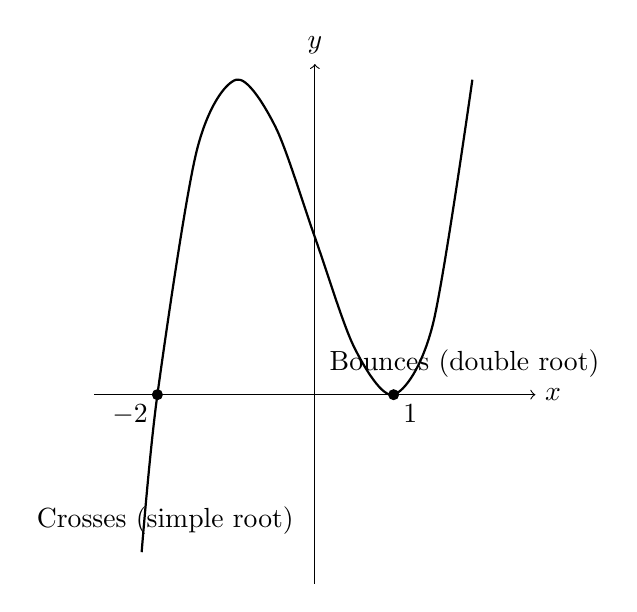
\begin{tikzpicture}[scale=1.0]
\draw[->] (-2.8,0) -- (2.8,0) node[right] {$x$};
\draw[->] (0,-2.4) -- (0,4.2) node[above] {$y$};
\draw[thick,smooth] plot coordinates {(-2.2,-2.0) (-2,0) (-1.5,3.1) (-1,4) (-0.5,3.4) (0,2) (0.5,0.6) (1,0) (1.5,0.9) (2,4)};
\fill (-2,0) circle (2pt) node[below left] {$-2$};
\fill (1,0) circle (2pt) node[below right] {$1$};
\node at (-1.9,-1.6) {Crosses (simple root)};
\node at (1.9,0.4) {Bounces (double root)};
\end{tikzpicture}
\end{center}

The second figure shows $y=(x+2)(x-1)^2$: it crosses at $-2$ and bounces at $1$. The graph openly reveals the secrets of the factorization.

Second, \textbf{degree and leading coefficient determine the ends' directions}. When the absolute value of $x$ is very large, lower-degree terms become negligible and the leading term $a_n x^n$ controls the behaviour. For even $n$, both ends point the same way (up if $a_n>0$, down if $a_n<0$); for odd $n$, they point in opposite directions. A by-product follows immediately: an odd-degree polynomial rises into the sky at one end and dives underground at the other, so it must cross the $x$-axis somewhere between them.

\begin{tuilun}
Every odd-degree polynomial has at least one real root.
\end{tuilun}

A rigorous proof needs the fact that a continuous curve cannot jump over the $x$-axis (the intermediate value theorem in Chapter 12 will make this precise), but the picture is persuasive: travelling from underground to the sky requires passing through ground level.

Third, \textbf{roots divide the curve into portions on which the sign stays fixed}. Want to solve $x^3-7x+6>0$? Factor it as $(x+3)(x-1)(x-2)$. The roots $-3$, $1$, and $2$ divide the number line into four intervals. Test one point in each to determine its sign, or construct a sign table. Each factor is positive to the right of its own root and negative to the left; the product's sign depends on whether the number of negative factors is even or odd.

\begin{center}
\begin{tabular}{ccccc}
\toprule
Interval & $x+3$ & $x-1$ & $x-2$ & Product $f(x)$ \\
\midrule
$x<-3$ & $-$ & $-$ & $-$ & $-$ \\
$-3<x<1$ & $+$ & $-$ & $-$ & $+$ \\
$1<x<2$ & $+$ & $+$ & $-$ & $-$ \\
$x>2$ & $+$ & $+$ & $+$ & $+$ \\
\bottomrule
\end{tabular}
\end{center}

Thus $f(x)>0$ holds for $-3<x<1$ or $x>2$. Read the table row by row, with no further equations to solve. A troublesome-looking inequality is settled by a map of the roots.

\section{A Rule from Three Points: Interpolation}

Return to the skatepark. The trajectory passes through $(0,2)$, $(1,5)$, and $(4,2)$; find the quadratic curve. Earlier we luckily guessed $y=-x^2+4x+2$. Now we will give a reliable method and prove uniqueness along the way.

The idea is surprisingly simple: \textbf{build components that are on duty at only one point}. Construct a quadratic polynomial $\ell_1(x)$ that equals $1$ at $x=0$ and $0$ at $x=1$ and $x=4$. The factor theorem handles the latter conditions immediately: $\ell_1$ must contain $(x-1)(x-4)$, so $\ell_1(x)=k(x-1)(x-4)$. Use its value $1$ at $0$ to determine $k$: substitution gives $k(0-1)(0-4)=4k=1$, so $k=\frac{1}{4}$ and
\[
\ell_1(x)=\tfrac{1}{4}(x-1)(x-4).
\]
Similarly, construct $\ell_2(x)=-\tfrac{1}{3}x(x-4)$, on duty at $x=1$ and equal to $0$ at the other two points (check that $\ell_2(1)=-\frac{1}{3}\cdot 1\cdot(-3)=1$), and $\ell_3(x)=\tfrac{1}{8}x(x-1)$, on duty at $x=4$.

Now, like a sound mixing desk, combine the three components according to their target heights:
\[
f(x) = 2\,\ell_1(x) + 5\,\ell_2(x) + 2\,\ell_3(x).
\]
Check: at $x=0$, $\ell_2$ and $\ell_3$ are $0$ while $\ell_1=1$, so $f(0)=2$. Similarly, $f(1)=5$ and $f(4)=2$. Expanding and combining gives $f(x)=-x^2+4x+2$, just as guessed, but now calculated. The same procedure works for any three points. Its name is \textbf{Lagrange interpolation}.

\begin{zhu}[Uniqueness]
Only one quadratic polynomial passes through these three points. If both $f$ and $g$ satisfy the requirements, consider $f-g$. It is zero at $0$, $1$, and $4$: a polynomial of degree at most $2$ has three roots! That contradicts the two-root bound unless $f-g$ is identically zero. The bound we just proved has immediately found a use.
\end{zhu}

In general, $n+1$ points with distinct horizontal coordinates determine exactly one polynomial of degree at most $n$. Fewer points leave the answer nonunique; more points may not all lie on any polynomial of the chosen low degree.

There is a subtle caution here: with more points, is higher degree always better? Quite the opposite. If measurements contain errors, as real measurements always do, a high-degree curve forced through every point can oscillate wildly between them and predict badly. Engineers usually prefer a lower-degree curve passing approximately through all the points. This is fitting, a close relative of interpolation. Interpolation insists on passing exactly through the points; fitting seeks the best overall match. Knowing which to use is a basic skill in the age of data.

\begin{lianjie}
Interpolation is far more than a geometry game. When a phone enlarges a photograph, interpolation computes the new pixels' colours. Animators draw only keyframes, and software interpolates the frames between them. Weather stations observe only selected cities, and interpolation fills out a national temperature map. More remarkably, error-correcting codes transmit data as values of a polynomial. Even if a few points are lost along the way, interpolation can reconstruct the entire polynomial. You use this every day when listening to music or scanning a QR code.
\end{lianjie}

\section{When Solutions Run Out: The Birth of $i$}

Now face this chapter's biggest stumbling block: $x^2+1=0$.

Over the real numbers it has no solution, since no real square is negative. Mathematicians centuries ago thought the same and consigned such equations to the wastebasket of meaninglessness. The turning point came in sixteenth-century Italy, where competitions to solve cubic equations revealed that solution formulas sometimes required square roots of negative numbers along the way. Strangely, if one \emph{pretended} those square roots existed and pressed on using ordinary rules, the imaginary parts eventually cancelled in pairs, and the resulting answer checked perfectly in the original equation!

This was awkward: a nonexistent number had become an indispensable bridge to a correct answer. Reject it, and real roots known to exist became inaccessible; accept it, and the calculation flowed. Mathematicians argued and doubted for more than a century. Some called these numbers sophistical quantities; others refused to write them. But their computational power was irresistible: results reached through imaginary numbers could be checked with real ones and repeatedly proved correct. After practice voted again and again, theory finally yielded. Mathematicians decided to recognize the bridge officially and grant it citizenship. Introduce a new number $i$ satisfying
\[
i^2 = -1.
\]
$i$ is not an inhabitant of the real number line; there is no place for it there. Where does it live? The answer is beautifully reassuring. Since real numbers fill a straight line, put $i$ \emph{outside} that line, at $(0,1)$ in a plane. Then a general complex number $a+bi$ is the point $(a,b)$: real numbers lie along the horizontal axis, and $i$ stands one unit up the vertical axis.

\begin{shuyu}{Complex Number}
Intuition: a point in the plane whose horizontal coordinate is the real part and whose vertical coordinate is the imaginary part.

Formal definition: a number of the form $a+bi$, where $a$ and $b$ are real and $i$ satisfies $i^2=-1$.

Example: $3-2i$ corresponds to $(3,-2)$; the real number $5$ is $5+0i$, and the purely imaginary number $2i$ is $0+2i$.
\end{shuyu}

All the rules for complex arithmetic follow from one principle: calculate as in ordinary algebra, replacing $i^2$ with $-1$ whenever it appears. Addition adds corresponding components: $(1+2i)+(3-i)=4+i$, represented geometrically by placing two arrows head to tail. Multiplication uses the distributive law:
\[
(1+2i)(3-i)=3-i+6i-2i^2=3+5i-2\times(-1)=5+5i.
\]
Each complex number $a+bi$ also has a mirror partner $a-bi$, called its \textbf{conjugate}. Their sum is $2a$, a real number; their product is $a^2+b^2$, a nonnegative real number equal to the squared distance from the origin. This partnership turns division into multiplication too: multiply numerator and denominator by the denominator's conjugate, and the denominator immediately becomes real.

\begin{center}
\begin{tikzpicture}[scale=1.4]
\draw[->] (-2.2,0) -- (2.4,0) node[right] {Real axis};
\draw[->] (0,-1.6) -- (0,1.9) node[above] {Imaginary axis};
\fill (1,0) circle (1.5pt) node[below right] {$1$};
\fill (-1,0) circle (1.5pt) node[below left] {$-1$};
\fill (0,1) circle (1.5pt) node[above right] {$i$};
\fill (0,-1) circle (1.5pt) node[below right] {$-i$};
\draw[->,thick] (0.75,0) arc (0:90:0.75);
\node at (0.95,0.7) {$\times i$};
\end{tikzpicture}
\end{center}

Complex multiplication has a geometrical interpretation: multiplying by $i$ rotates a point $90^\circ$ anticlockwise about the origin. $1\times i = i$ turns rightward into upward; $i\times i = i^2 = -1$ turns another $90^\circ$ to the left. A square root of a negative number turns out to be the square root of the action of making a half-turn. How natural!

With $i$, the equation $x^2+1=0$ has roots $\pm i$, and the quadratic formula gives, for $x^2+x+1=0$,
\[
x=\frac{-1\pm\sqrt{-3}}{2}=-\frac{1}{2}\pm\frac{\sqrt{3}}{2}i.
\]
Remember the earlier shortfall? These two complex roots sum to exactly $-1$ and multiply to exactly $1$. Vieta's relations still hold in the complex world. More astonishing is the following fact:

\begin{dingli}[The Fundamental Theorem of Algebra]
Every polynomial of degree $n$ with complex coefficients, where $n\ge 1$, has at least one complex root. Repeated application of the factor theorem then splits it into a product of $n$ linear factors: it has exactly $n$ roots, counting repeated roots according to their multiplicities.
\end{dingli}

The proof goes beyond this book's tools. It requires some analysis or topology; university courses in complex analysis offer particularly elegant proofs. But its message is clear: \textbf{complex numbers make degree and number of roots match perfectly}. Earlier qualifications---odd degree guarantees a real root, a quadratic may have none---disappear in the complex world. A degree-$n$ equation always has exactly $n$ solutions, no more and no fewer. Introducing a new kind of number brings striking order.

Looking back, number systems have expanded along a familiar road: measuring land required fractions; accounting for debts required negative numbers; measuring diagonals required irrational numbers; solving equations required complex numbers. Each time solutions run out, mathematics is knocking on a door. Behind it waits a larger number system and a tidier collection of theorems.

\begin{pandeng}
Further ahead you will encounter the \textbf{remainder theorem} ($f(a)$ is exactly the remainder when $f$ is divided by $x-a$), the general \textbf{Lagrange interpolation formula}, the \textbf{conjugate root theorem} (nonreal roots of equations with real coefficients come in pairs), and \textbf{roots of unity} in the complex plane. Farther still stands a major question: why is there no general solution formula for equations of degree five and higher? Its answer gave birth to a subject that studies equations through symmetry: \textbf{group theory}.
\end{pandeng}

\section{Hands-on Time}

\begin{shiyan}
\textbf{Experiment 1: Predicting a Graph from Its Roots.} Without using a calculator, answer these questions from $f(x)=(x+2)(x-1)(x-3)$ alone. (1) At which three positions does the curve meet the $x$-axis, and does it cross or bounce? (2) Where do its ends point for very large positive and negative $x$? (3) Mark the intervals where $f(x)>0$ and $f(x)<0$ on a number line. Then plot points, sketch the curve, and check each prediction.

\textbf{Experiment 2: Interpolation by Hand.} Take $(0,1)$, $(2,3)$, and $(3,1)$. Following the text, construct three components $\ell_1$, $\ell_2$, and $\ell_3$, each on duty at one point, and combine them by height to obtain $f(x)$. Expand and substitute all three points to check. Then choose another horizontal coordinate, such as $x=1$, calculate its function value, plot it, and see whether the curve smoothly joins your points.

\textbf{Experiment 3: Vieta the Detective.} Ask a classmate to choose two integer roots of a quadratic secretly and tell you only their sum and product. Use Vieta's relations to reconstruct the equation, then solve it to check. Switch roles for three rounds and consider what it means for coefficients to see only symmetric information.
\end{shiyan}

\begin{toolbox}
This chapter's new tools:
\begin{itemize}
\item \textbf{Polynomials, coefficients, and degree}: a large class of expressions becomes one unified object of study.
\item \textbf{The factor theorem}: roots and linear factors translate into each other; finding one root lowers the equation's degree by one.
\item \textbf{Bounds on roots}: a degree-$n$ polynomial has at most $n$ real roots; an odd-degree polynomial has at least one.
\item \textbf{Vieta's relations}: coefficients are symmetric functions of roots, revealing information without solving the equation.
\item \textbf{Multiplicity and graphs}: simple roots cross the axis, repeated roots touch and bounce; the leading term determines the ends' directions.
\item \textbf{Lagrange interpolation}: $n+1$ points uniquely determine a rule of degree at most $n$.
\item \textbf{Complex numbers}: $i^2=-1$; in the complex world, a degree-$n$ equation has exactly $n$ solutions.
\end{itemize}
\end{toolbox}

\section*{Questions to Think About}

\textbf{Observation}
\begin{sikao}
\item Examine sketches of $y=x^2$, $y=x^3$, $y=x^4$, and $y=x^5$. What patterns distinguish even and odd degrees for very large positive and negative $x$? Hint: consider only the leading term, treating other terms as negligible small fluctuations.
\item Sketch $y=(x-1)^3$. The point $x=1$ is a triple root: does the curve cross or bounce there? Hint: an odd power changes sign, but growth flattens near the root. Plot $x=0.5$, $1$, and $1.5$ and look closely.
\end{sikao}

\textbf{Proof}
\begin{sikao}
\item Prove that if $x^2+bx+c=0$ has two real roots, they have the same sign when their product is positive and opposite signs when it is negative. Hint: use Vieta's relation $\alpha\beta=c$ directly.
\item A cubic polynomial $f(x)$ satisfies $f(1)=f(2)=f(3)=0$ and $f(0)=6$. Find $f(4)$. Hint: the factor theorem determines the form of $f$ up to one unknown coefficient.
\end{sikao}

\textbf{Challenge}
\begin{sikao}
\item Use $i^2=-1$ to calculate $(1+i)^2$ and $(1+i)^4$. Hint: plot each result in the complex plane and observe what happens to distance from the origin and angle at each squaring. This quietly echoes the rule that multiplying by $i$ rotates by $90^\circ$.
\item Prove that at most one polynomial of degree at most $n$ passes through $n+1$ points with distinct horizontal coordinates. Hint: follow the uniqueness note in the text, consider the difference of two candidates, and count its roots.
\end{sikao}

\section*{The Door to the Next Chapter}

Symmetry has appeared quietly several times in this chapter. In Vieta's relations, $\alpha+\beta$ and $\alpha\beta$ remain unchanged when the two roots are exchanged; coefficients see only symmetric information about roots. And the ultimate question---why cubics and quartics have solution formulas but equations of degree five and higher do not---eventually receives this answer: \textbf{the symmetries among the roots of a quintic are too complicated to express through finitely many root extractions}.

Giving an equation's roots a symmetry check sounds extraordinary. But symmetry itself can be a precisely defined mathematical object on which we calculate. How many reflections and rotations does a square have? How do these operations combine? Does reflecting and then rotating give the same result as rotating and then reflecting? Next chapter we will turn symmetry from an adjective into a noun, from an impression into a structure, and follow it to the heart of modern algebra: groups.
